\documentclass[12pt,a4paper,roman]{article}
\usepackage[utf8]{inputenc}
\usepackage[margin=2.5cm]{geometry}

\title{Research in Data Science and Methodology}
\author{%
\textsc{Enseignant : Oliver Schwander} \\% Your name
\textsc Jean Soler, Nicolas Castanet% Your email address
%\and % Uncomment if 2 authors are required, duplicate these 4 lines if more
%\textsc{Jane Smith}\thanks{Corresponding author} \\[1ex] % Second author's name
%\normalsize University of Utah \\ % Second author's institution
%\normalsize \href{mailto:jane@smith.com}{jane@smith.com} % Second author's email address
}
\date{October 2020}

\usepackage{natbib}
\usepackage{graphicx}
\begin{document}
\maketitle
\begin{abstract}
Ce rapport à pour but d'établir une analyse préliminaire du dataset UC2017 dans le cadre d'un projet pour l'UE d'initiation à la recherche et méthodologie en science des données.
\end{abstract}
\section{Introduction}
Le dataset UC2017 est présenté dans l'article [1], il est constitué d'un ensemble de geste réalisés à la mains par plusieurs utilisateurs. Il à pour but l'interaction des hommes avec des robots à travers la classification de gestes simples par des algorithmes de classifications. 
\newline
Les données propres aux gestes ne sont pas acquis par vidéo mais par des capteurs magnétiques que l'utilisateur porte directement.
Voici les ambitions des ingénieurs pour ce dataset :
\begin{itemize}
    \item Fournir un dataset complet pour l'interaction homme machine.
    \item Avoir de la variance du aux utilisateurs.
    \item Fournir des gestes représentatifs de gestes qui pourraient être exécutés tous les jours et dans n'importe quelles conditions.
\end{itemize}

\section{Dataset UC2017}
\subsection{Description générale}
Le dataset est constitué de deux types de gestes, les gestes statiques (SG) et les gestes dynamiques (DG). Il compte 24 différents SG et 10 DG. Nous nous intéresserons principalement aux SG dans cette analyse préliminaire. 
\newline
\textbf{Voici la campagne de réalisation des gestes}:
\begin{itemize}
    \item SG : 8 utilisateurs, pour un total de 100 répétitions pour les 24 gestes = 24x100 = 2400 exemples.
    \item DG : 6 utilisateurs, pour un total de 131 répétitions pour les 10 gestes = 10x131 = 1310 exemples.
\end{itemize}
Les gestes sont réalisés de la main gauche par des droitiers ce qui induit moins d'assurance dans les gestes. Ceci et la variété des utilisateurs induit de la variance dans les données.

\newpage
On remarque également que chaque utilisateur à réalisé chaque type de geste un nombre identique de fois mais que certains utilisateurs ont réalisé au total beaucoup plus de geste que d'autres. En voici l'illustration sur la répartition des 2400 exemples de SG avec la classe des gestes :

\begin{figure}[h!]
\centering
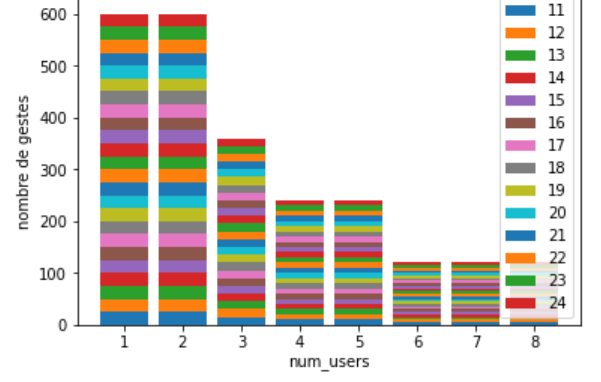
\includegraphics[scale=0.5]{comptage.png}
\caption{nombre de gestes réalisés par chaque utilisateurs, les différentes couleurs correspondants au classes des 24 SG.}
\label{fig:universe}
\end{figure}

Le dataset UC2017 est donc équilibré en classes, avec une variance multi-factorielle (plusieurs utilisateurs, gestes exécutés de manière variables, ordre d'exécution des gestes aléatoire, absence de calibrage, imprécision du placement des capteurs ...). 
\newline
Les données sont également biaisées par le manque de proportion des utilisateurs dans la réalisation des gestes : On voit ci-dessus que 1200 gestes sur 2400 ont été réalisés par 2 utilisateurs sur 8. Les algorithmes d'apprentissage seront donc beaucoup pus sensible à une exécution des gestes propre à ces deux utilisateurs (morphologie, habitude de mouvement, etc ...). 
Afin de mettre en évidence ce phénomène nous avons réalisé une analyse en composantes principales (ACP) de 2 composants  afin d'observer la variance des données en fonction des utilisateurs.

\begin{figure}[!h]
 	\begin{center}
 	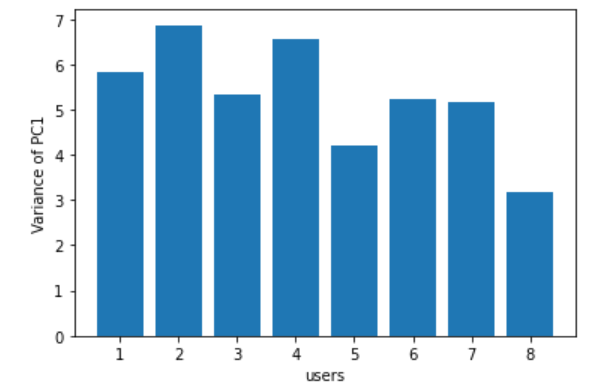
\includegraphics[scale=0.35]{pc1.png}
 	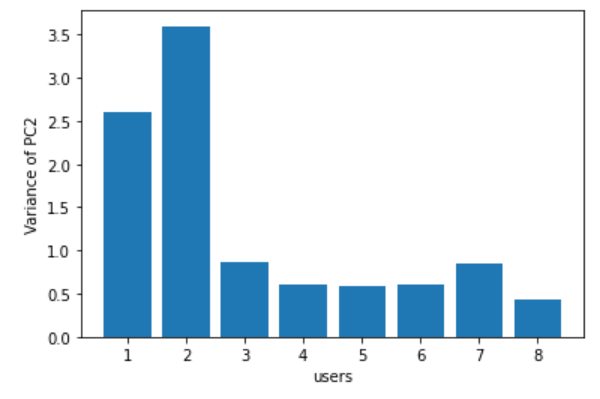
\includegraphics[scale=0.35]{pc2.png}
 	\caption{Variance des principaux composants 1 et 2 en fonction de l'utilisateur.}
 	\end{center}
\end{figure}
On observe que pour le composant principal 2, l'essentiel de la variance provient des utilisateurs 1 et 2. On en déduit qu'une grande partie de la variance des données est du à ces deux utilisateurs.


\subsection{Caractéristiques des données}

Les SG sont représentés par les caractéristiques de la mains à un instant donné tandis que les DG sont représentés par les caractéristiques de la mains au court du temps (le temps de réalisation d'un DG n'est pas fixe).
\newline
Les caractéristiques des gestes sont obtenues à l'aide d'un gant et d'un traceur magnétique. \textbf{Le gant à pour but de capter la forme, la position et l'orientation de la main}. Il possède 22 capteurs situés au niveau des articulations des doigts, du poignet et de la paume, chaque capteurs envoi donc un signal proportionnel à l'angle de l'articulation correspondante $g1, g2, ..., g22$.
\newline
\textbf{Le traceur magnétique de son coté à pour but de mesurer la position et l'orientation du poignet dans l'espace}. Il en résulte 6 nouveaux signaux : $l1, l2, l3$ correspondant à la position dans l'espace et $l4, l5, l6$ correspondants à différentes angles du poignet dans l'espace.
\newline
Un geste statique est donc un ensemble de ces 28 caractéristiques, tandis qu'un geste dynamique de dimension 28 x le nombre d'enregistrement au court du temps.

\section{Classification}
\subsection{tâches machine-learning}
Plusieurs taches de classification sont envisageables pour ce dataset. La plus évidente serait la classification de geste sur tous les utilisateurs afin de maximiser la variance des données, afin d'en faire un système de reconnaissance universel. La machine serait idéalement capable de reconnaître les gestes de n'importe qui et dans n'importe quelle conditions. On entraînerait alors un algorithme de classification sur les données venant de tous les utilisateurs.
\vspace{0.1cm}

Une deuxième tache est la classification de geste pour un seul utilisateur, afin de concevoir un système personnalisé. Les données des utilisateurs 1 et 2 sont peuvent être suffisantes et suffisamment variées afin de pouvoir entraîner un algorithme de classification. Des stratégies d'augmentation de données sont envisageables pour cette tâche.
\vspace{0.1cm}

Ce dataset contient le numéro de l'utilisateur pour chaque geste, on pourrait donc envisager de retourner le problème en réalisant de la classification d'utilisateurs. La classe du geste deviendrait une caractéristique. Les motivations de cette tache sont complètement différentes de celle pour la reconnaissance de geste : il ne s'agit plus d'interaction homme-machine, mais plutôt d'un objectif de reconnaissance d'individus pour la sécurité ou la surveillance. Ce problème serait cependant non proportionnel, on pourrait donc dans un premier temps considérer les gestes des utilisateurs 1 et 2. En effet, ces utilisateurs ont fournit chacun 600 gestes, une première tentative serait de reconnaître si un geste est réaliser par l'un ou l'autre.

\subsection{Choix des algorithmes et pré-traitement des données}
Le but sera dans un premier temps d'explorer différents types d'algorithmes de classification en essayant de reproduire les baseline établis dans l'article [1]. Nous évaluerons la performance d'algorithmes classiques comme le SVM, les K plus proches voisins ou les arbres de décisions en nous inspirant des travaux réalisés dans [1]. 
\newpage

Pour les tâches de reconnaissance de gestes, nous devons également garder à l'esprit que le but de ce dataset est l'interaction homme-machine en direct. Si le système est entraîné préalablement, alors le temps d'entraînement n'est pas à prendre en considération. Si le système vient à être entraîné en direct, alors un algorithme avec un entraînement rapide est à privilégier. Dans les deux cas un algorithme entraîné doit être capable de calculer rapidement la classe du geste. Un algorithme comme les KNN, devant calculer à chaque nouveaux geste ses K plus proches voisins, sera peu efficace pour la reconnaissance en ligne.








\bibliographystyle{plain}
\bibliography{references}
[1] Miguel Simão, Olivier Gibaru et Pedro Neto \textit{"Online Recognition of Incomplete Gesture Data to Interface Collaborative Robots"} IEEE Transactions on Industrial Electronics - 2019
\end{document}
